\documentclass{standalone}
\usepackage{tikz}
\begin{document}
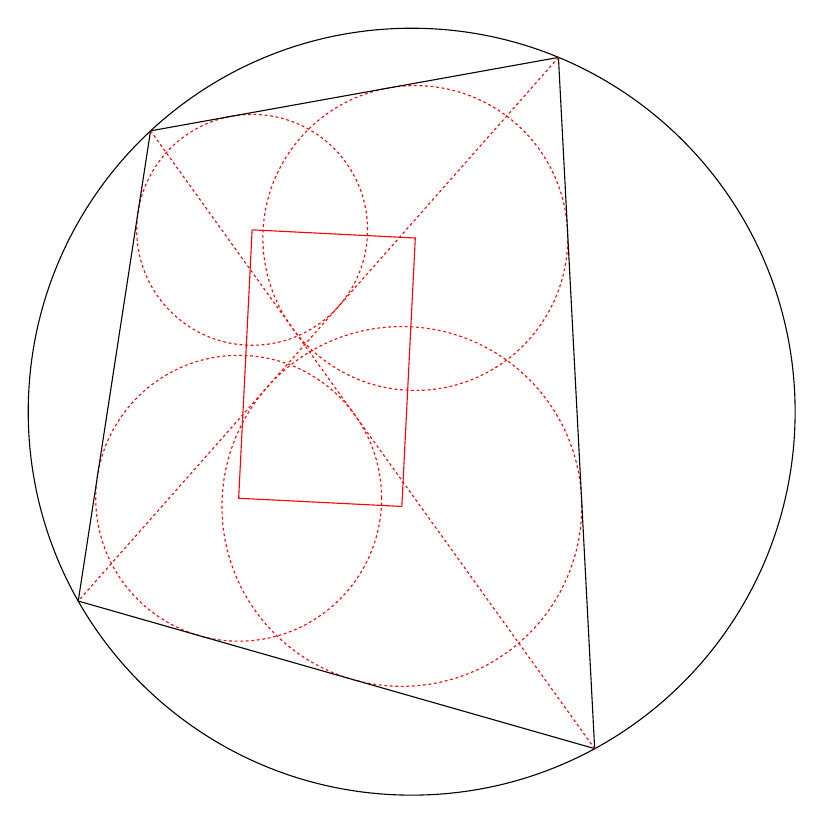
\begin{tikzpicture}[x=1pt,y=1pt]
\draw (148.61,-152.51) circle (138.56);
\draw[red, dash pattern=on 1pt] (149.92,-89.76) circle (55.07);
\draw[red, dash pattern=on 1pt] (86.09,-183.79) circle (51.65);
\draw[red, dash pattern=on 1pt] (90.96,-86.80) circle (41.71);
\draw[red, dash pattern=on 1pt] (145.06,-186.75) circle (65.00);
\draw (201.64,-24.50) -- (54.25,-51.03) -- (28.12,-220.94) -- (214.73,-274.27) -- cycle;
\draw[red, dash pattern=on 1pt] (54.26,-51.03) -- (214.73,-274.28);
\draw[red, dash pattern=on 1pt] (201.65,-24.50) -- (28.12,-220.94);
\draw[red] (90.96,-86.80) -- (86.09,-183.79) -- (145.05,-186.75) -- (149.92,-89.76) -- cycle;
\end{tikzpicture}
\end{document}
